\documentclass[onecolumn]{article}
%\usepackage{url}
%\usepackage{algorithmic}
\usepackage[a4paper]{geometry}
\usepackage{datetime}
\usepackage[margin=2em, font=small,labelfont=it]{caption}
\usepackage{graphicx}
\usepackage{mathpazo} % use palatino
\usepackage[scaled]{helvet} % helvetica
\usepackage{microtype}
\usepackage{amsmath}
\usepackage{subfigure}
\usepackage{hyperref}
\hypersetup{
    colorlinks=true,
    linkcolor=blue,
    filecolor=magenta,      
    urlcolor=blue,
}
%\urlstyle{same}
% Letterspacing macros
\newcommand{\spacecaps}[1]{\textls[200]{\MakeUppercase{#1}}}
\newcommand{\spacesc}[1]{\textls[50]{\textsc{\MakeLowercase{#1}}}}

\title{\spacecaps{Project module report: Argumentation Mining }\\ \normalsize \spacesc{University of Potsdam, Winter semester 2017/18} }

\author{Oğuz Serbetci\\Maria Stazherova}
%\date{\today\\\currenttime}
\date{\today}

\begin{document}
\maketitle

\begin{abstract}

Structure prediction on "microtext" corpus. We used Keras Functional API throughout the project. The code can be found on GitHub under \url{https://github.com/oguzserbetci/argmin2017}

\end{abstract}


\section{Data \& Task}
We worked with the arg-microtext corpus \cite{peldszus2015annotated}, which contains 112 short argumentative texts 
(originally in German and profesionally translated to English). Later we received preliminary annotations of the new microtexts
and could incorporate them into the project.

\begin{figure}[h]
    \centering
    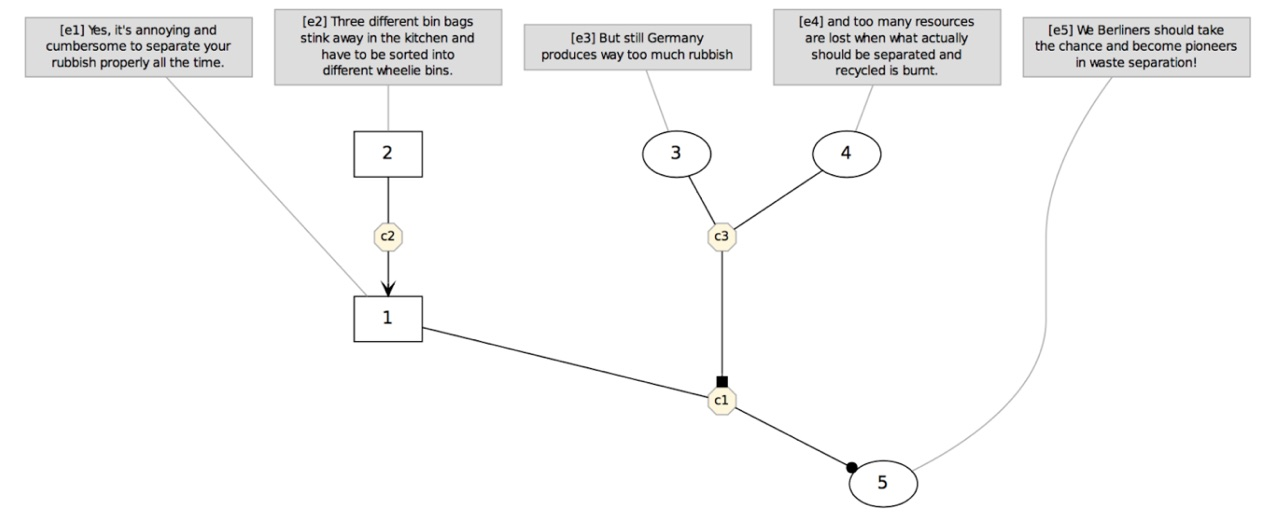
\includegraphics[width=0.8\linewidth]{fig/microtext.jpg}
    \caption{One example from arg-microtext corpus and its argumentation graph.
            \\Round nodes are proponent's nodes, square ones are opponent's nodes. The arcs connecting the nodes represent different supporting and attacking moves.}
    \label{fig:microtext}
        \end{figure}

As can be seen in the figure \ref{fig:microtext}, each text in the corpus is a single tree and argument components (ACs) are either claims, or premises. 
Each text in our corpus had only one claim. 
We decided to concentrate on two tasks: classifying the type of an AC (claim or premise), and determining the links between ACs.

\section{Approach}
\subsection{Inspiration}
Having found the paper ``Here's My Point: Joint Pointer Architecture for Argument Mining'' by Potash et al. \cite{potash2017here}, we agreed that it
would be good to try and reproduce the architecture and results from this paper, especially because the authors claimed they achieved
state-of-the-art results. The authors used a seq2seq (sequence-to-sequence) architecture with attention, called
Pointer Networks, which they then extended to a ``joint model'' (architecture can be seen in figure \ref{fig:joint}) which was able to simultaneously address the link extraction task and the classification of argument components. 

\begin{figure}[h]
    \centering
    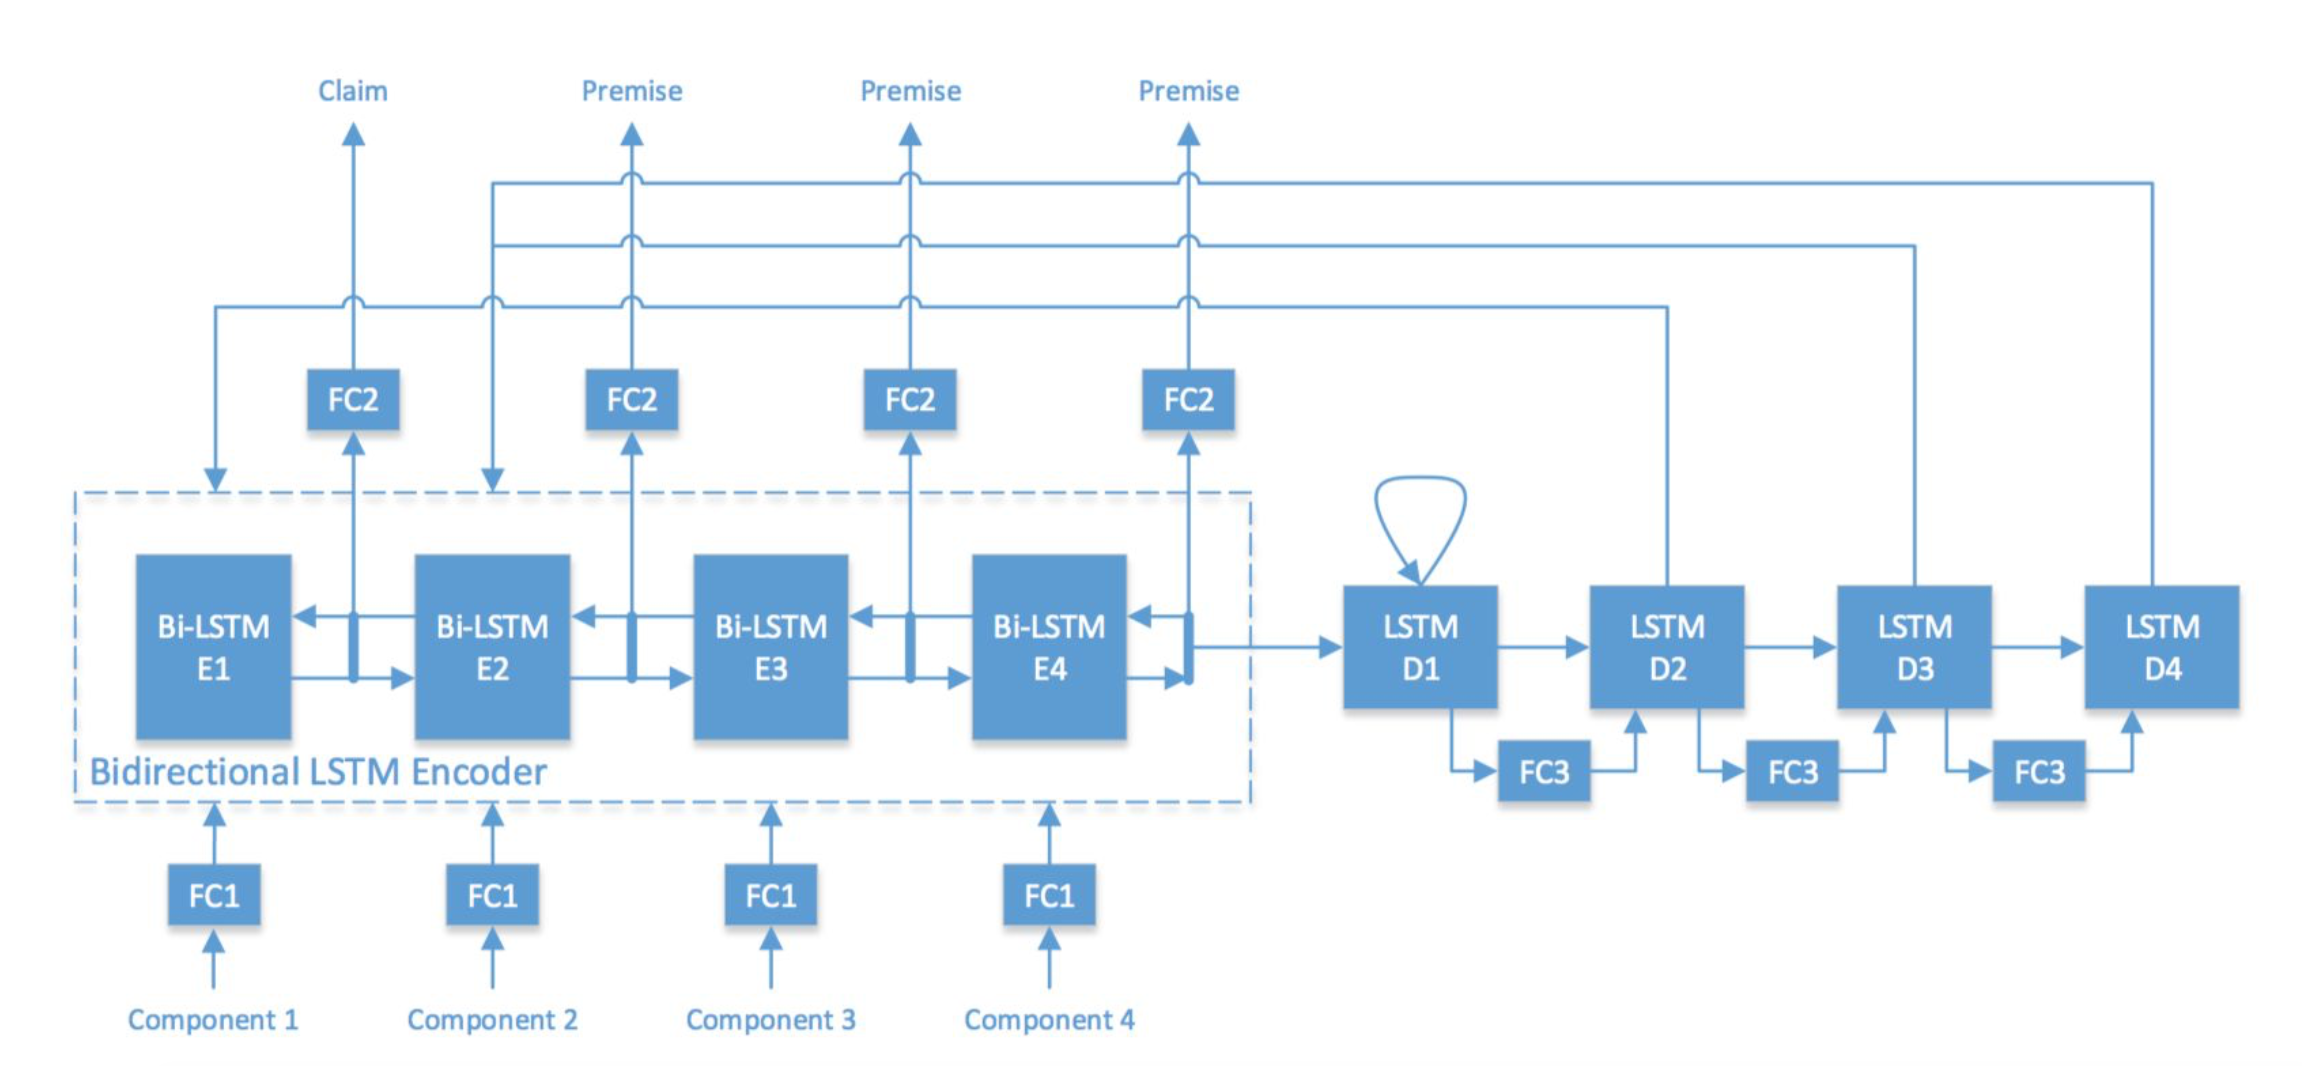
\includegraphics[width=0.8\linewidth]{fig/joint.png}
    \caption{Architecture of joint model from the paper by Potash et al. \cite{potash2017here}, applied to an example of argument structure with four ACs.
            \\D1 pointing to itself denotes that it has no outgoing link and is the head of a tree.}
    \label{fig:joint}
        \end{figure}

\subsection{Workflow}
We started our work by doing the data preprocessing and creating simple bag-of-words vector representations of argument components. 
After that we implemented a pointer network with one-directional encoder for the single task (determining the links between ACs).
We sticked to the regularization techniques and their strength, as it was applied in the paper \cite{potash2017here}. 

Our next step was to implement the fully-connected inputs (add a fully connected layer to encoder input,
as well as to the decoder input), to make the LSTM bidirectional and to use all applicable to our corpus features from the paper: structural feature 
(binary, is the AC the first one in text or not), bag-of-words over the whole data and embedding representations (average, min and max pooling
of word vectors of tokens). 

After that we moved further on implementing the joint model architecture with an additional task of classifying the type of AC (claim or premise). 
The diagram we made for better understanding of the architecture can be seen in figure \ref{fig:our-model}.

We implemented 5-fold cross-validation for hyperparameter tuning and evaluation.
\begin{figure}[h]
    \centering
    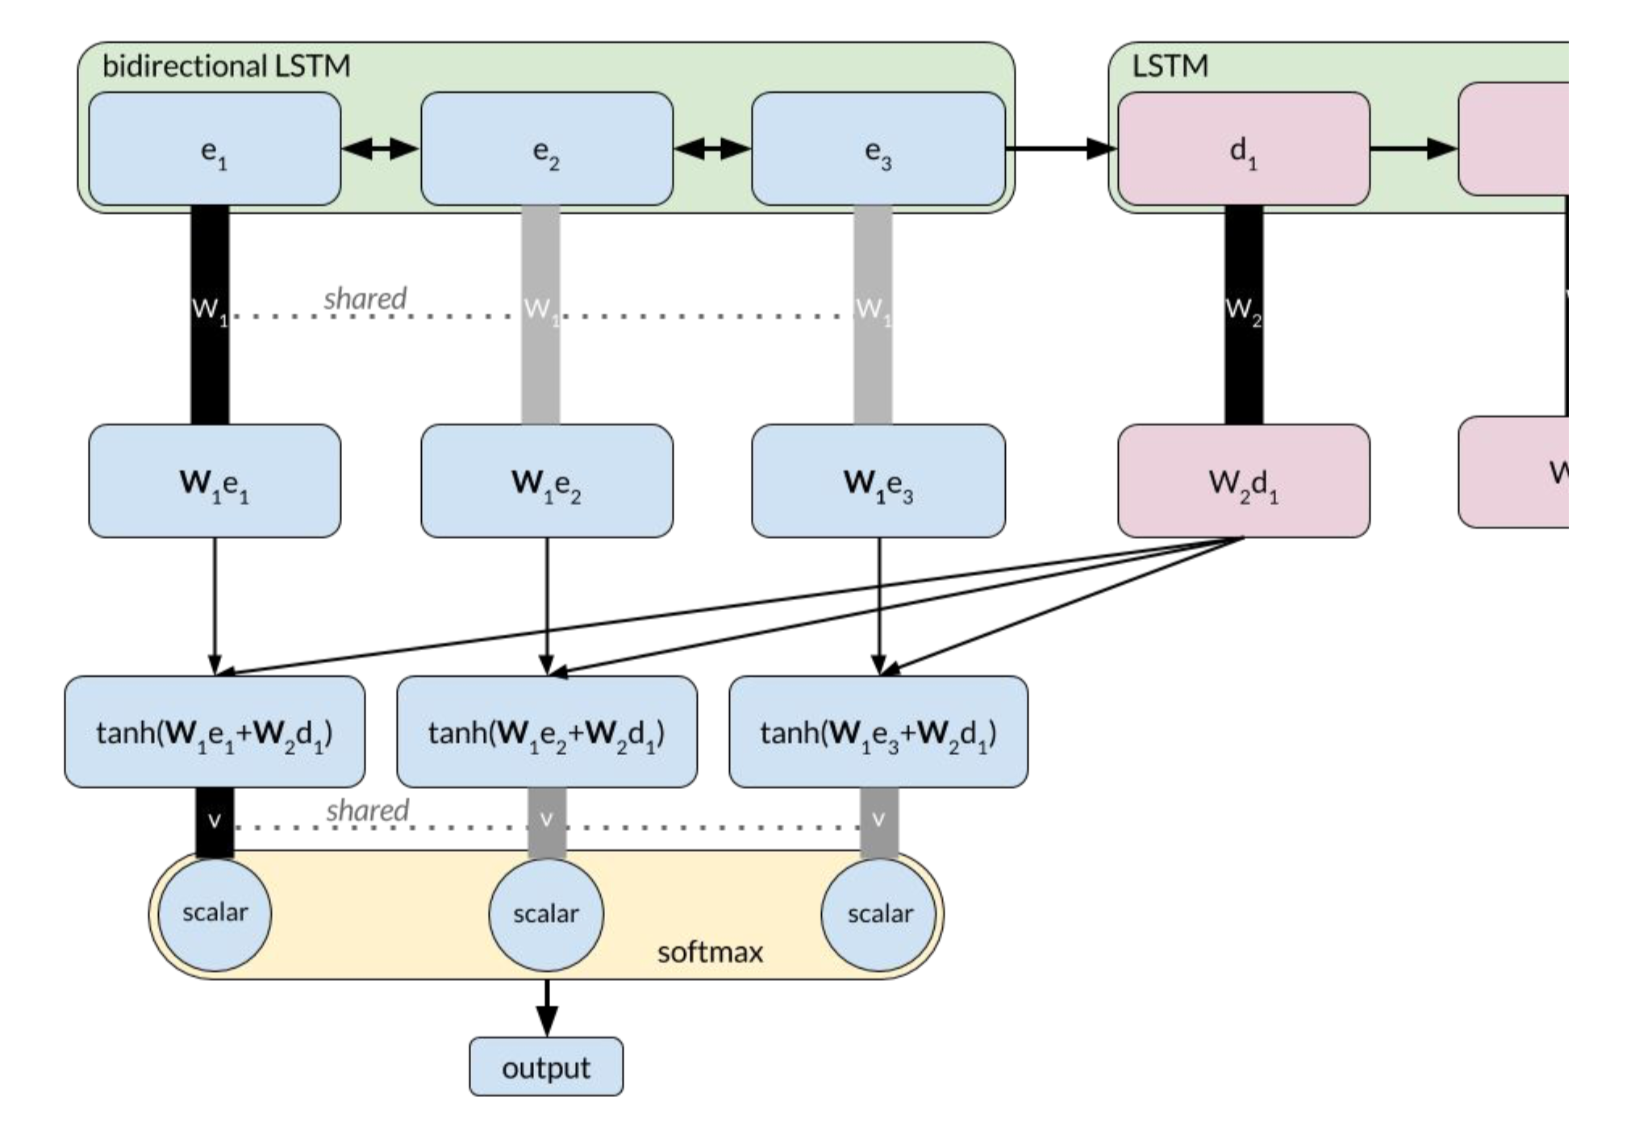
\includegraphics[width=0.8\linewidth]{fig/architecture.png}
    \caption{Essential part of our architecture of the joint model}
    \label{fig:our-model}
        \end{figure}

\subsection{Challenges}
While working on the project, we encountered some difficulties and made some errors that we then corrected. The first one 
was to think of the proper way to pad input sequences so that they have the same length. When we implemented the joint model, 
we decided to filter out examples that were longer than 6 in length, because of the distribution of document length in the corpus, which
can be seen in the figure \ref{fig:length}. Documents were padded with zeros, e.g. link conversion would look like following: 
from 1,1,2 we would get [1,0,0,0][1,0,0,0][0,1,0,0][0,0,0,0].


\begin{figure}[h]
    \centering
    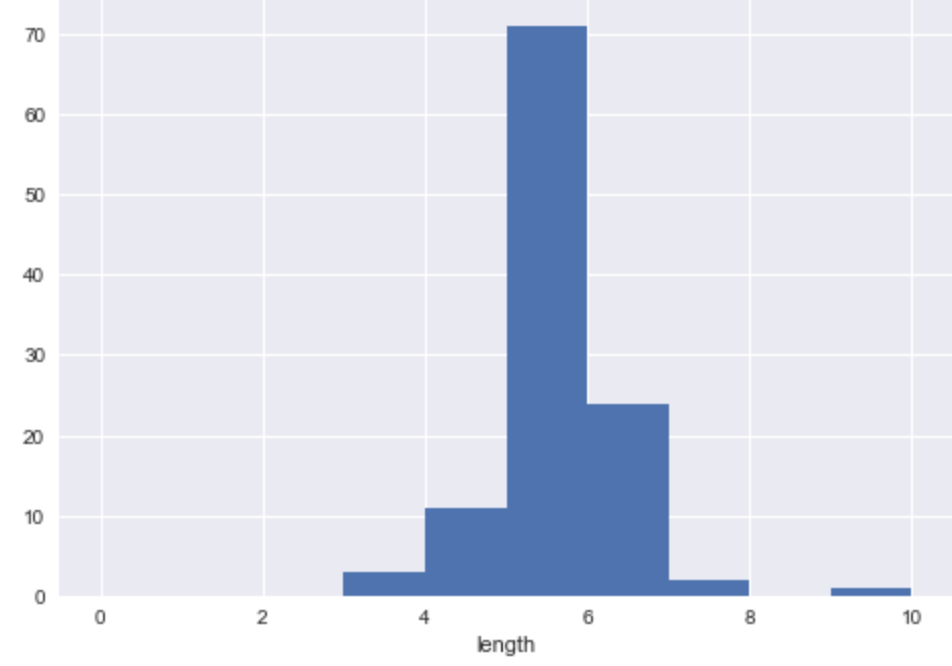
\includegraphics[width=0.4\linewidth]{fig/doc-length.png}
    \caption{Distribution of document length in the corpus}
    \label{fig:length}
        \end{figure}




\section{Results}
Intermediate 5-fold cross validation on the joint model yielded \textbf{0.603(+/-0.086)} validation accuracy using all features. 

results!

\section{Conclusion}
future ideas and improvements

\nocite{*}
\bibliographystyle{plain}
\bibliography{references}
\end{document}
